\subsection{HiPhyBoost: transfer of discrimination}\label{sec:res_hiphy}
Estimating event offsets jointly with the shared response improves transfer in most events. In the same leave-one-event-out design, HiPhyBoost reaches a median AUC of 0.833 and a median AP lift of 4.1, compared with 0.805 and 3.4 for PC-GBM and 0.790 and 3.9 for the unconstrained GBM (Table~\ref{tab:hiphy}). The ablation with offsets fixed at zero keeps the Newmark anchor, the constraints and the larger number of trees (700 instead of 400) but removes the offsets. It reaches 0.810, practically equal to PC-GBM (mean difference $+0.001$). The gain is therefore due to the offsets, not to the physics anchor or the larger tree budget. The spatial block bootstrap shows that HiPhyBoost is significantly better than PC-GBM at Kaik\={o}ura ($+0.030$; 95\% interval $0.021$--$0.038$), Northridge ($+0.019$), Denali ($+0.042$), Porgera ($+0.044$) and Palu ($+0.049$). It is equivalent at Niigata and Iwate, and slightly worse at Ays\'en ($-0.025$) and Cinchona ($-0.013$), the two events with very weak ShakeMap shaking. These bootstrap intervals describe uncertainty within each event. Treating the nine events as the units of replication, HiPhyBoost is better than PC-GBM in six of nine events (mean $\Delta$AUC $+0.016$, median $+0.019$), but the difference is not significant with nine events (Wilcoxon signed-rank $p=0.16$; against the unconstrained GBM $p=0.07$; against the global LR $p=0.004$). The improvement is therefore consistent but modest, and it should be confirmed with further inventories. For Kaik\={o}ura, the model trained only on the eight other Pacific Rim earthquakes reaches AUC 0.917 and concentrates landslides 12.7 times more than random. This is close to the local model fitted to the Kaik\={o}ura inventory itself (AUC 0.934, AP lift 16.8), and the predicted landslide density at 2~km resolution agrees with the GNS inventory with Spearman $\rho=0.61$ (Figure~\ref{fig:kaikoura}). Similar rank agreement at 2~km is obtained for Northridge, Iwate, Porgera and Palu ($\rho=0.51$--$0.64$; Figure~\ref{fig:maps}).

Why does modelling the level improve the ranking? In a pooled model, an event with a high base rate, such as Cinchona or Niigata, pulls the shared response towards predictors that happen to separate that event from the others, for example low PGV or particular terrain textures. These predictors then act as proxies for ``being in a landslide-prone earthquake'' rather than for ``being a susceptible hillslope''. Once each event has its own offset, between-event differences are absorbed by $b_e$, and the trees are fitted to within-event contrasts, which are the contrasts that matter when ranking hillslopes in a new earthquake. The two events where HiPhyBoost loses are those where within-event shaking contrasts are weakest (Supplementary Figure~S1): ranking there depends almost entirely on terrain, and pooling information on the base rate from the other events helps PC-GBM slightly.

\begin{table*}[t]\centering\small
\caption{Leave-one-event-out transfer of HiPhyBoost. AUC of the transferred PC-GBM, of HiPhyBoost without event offsets (ablation) and of the full HiPhyBoost ($^{*}$: 95\% block-bootstrap interval of the difference from PC-GBM excludes zero); AP lift; ratio of predicted to observed landslide cells for the HiPhyBoost point forecast ($E/O$); 90\% zero-shot predictive interval of $E/O$ and whether it contains 1.}\label{tab:hiphy}
\resizebox{\textwidth}{!}{\begin{tabular}{lrrrrrrlc}\toprule
 & \multicolumn{3}{c}{AUC} & \multicolumn{2}{c}{AP lift} & & \multicolumn{2}{c}{Zero-shot 90\% interval}\\\cmidrule(lr){2-4}\cmidrule(lr){5-6}\cmidrule(lr){8-9}
Event & PC-GBM & No offsets & HiPhyBoost & PC-GBM & HiPhyBoost & $E/O$ & $E/O$ interval & covers\\\midrule
Kaik\={o}ura 2016 (NZ) & 0.887 & 0.888 & \textbf{0.917}$^{*}$ & 9.2 & 12.7 & 1.06 & [0.060, 15.9] & yes\\
Northridge 1994 (USA) & 0.814 & 0.815 & \textbf{0.833}$^{*}$ & 5.0 & 6.1 & 0.46 & [0.026, 7.5] & yes\\
Niigata-Chuetsu 2004 (JP) & 0.788 & 0.794 & \textbf{0.784} & 3.2 & 3.0 & 0.13 & [0.008, 1.9] & yes\\
Iwate-Miyagi 2008 (JP) & 0.833 & 0.835 & \textbf{0.834} & 5.6 & 5.4 & 1.12 & [0.052, 19.2] & yes\\
Ais\'{e}n 2007 (CL) & 0.760 & 0.747 & \textbf{0.734}$^{*}$ & 3.3 & 2.8 & 0.15 & [0.008, 3.0] & yes\\
Denali 2002 (USA) & 0.805 & 0.810 & \textbf{0.848}$^{*}$ & 3.4 & 4.1 & 33.68 & [4.114, 241.7] & no\\
Cinchona 2009 (CR) & 0.774 & 0.776 & \textbf{0.760}$^{*}$ & 2.9 & 2.8 & 0.02 & [0.002, 0.2] & no\\
Porgera 2018 (PNG) & 0.872 & 0.877 & \textbf{0.916}$^{*}$ & 9.1 & 13.0 & 6.12 & [0.396, 79.7] & yes\\
Palu 2018 (ID) & 0.730 & 0.734 & \textbf{0.780}$^{*}$ & 2.5 & 3.7 & 1.24 & [0.065, 20.9] & yes\\
\midrule Median & 0.805 & 0.810 & 0.833 & 3.4 & 4.1 & 1.06 & & 7/9\\
\bottomrule\end{tabular}}\end{table*}


\subsection{Event offsets as a geoscientific quantity}\label{sec:res_offsets}
Fitted on all nine events, the offsets span 5.7 log-odds units, from $b=-3.15$ at Denali to $+2.59$ at Cinchona ($\tau=1.69$; Figure~\ref{fig:offsets}a). In other words, with terrain and computed Newmark displacement held equal, the odds of a landslide cell were about 300 times higher at Cinchona than at Denali. Offsets are strongly positive for Cinchona ($+2.6$) and Niigata-Chuetsu ($+1.7$) and moderately positive for Northridge ($+0.7$). They are close to zero for Ays\'en, Iwate, Kaik\={o}ura and Palu, and strongly negative for Porgera ($-1.6$) and Denali ($-3.2$). The offsets are stable across the leave-one-event-out folds (standard deviation of each event's offset across the eight folds in which it is a training event: 0.18--0.33 log-odds units, small compared with the 5.7-unit spread between events), so they are a robust property of the data, not an artefact of a particular fit. Their interpretation is discussed in Section~\ref{sec:disc}.

\subsection{Zero-shot forecasts of the landslide total}
Without any mapped landslide, the transferred point forecast of HiPhyBoost (the offset set to the prior median; the Bayesian predictive mean is a poor point forecast because the lognormal-like uncertainty of the total makes it overpredict, median $E/O=3.7$) is within a factor of two of the observed number of landslide cells in three events (Iwate, Kaik\={o}ura, Palu), compared with four for PC-GBM. Neither model can predict the base rate of an unseen earthquake, because the offsets are not explained by the inputs. The value of the Bayesian formulation is that it makes this ignorance explicit. The 90\% predictive interval of the landslide total spans a factor of 60--390, and it contains the observed total in seven of nine events (Figure~\ref{fig:offsets}b). Such wide intervals are only weakly informative, but they are honest. Replacing the normal prior by a Student-$t$ predictive that accounts for estimating $\mu$ and $\tau$ from eight events widens them further (median factor 850) without changing the coverage. The two misses are Cinchona, observed above the interval, and Denali, observed below it, the events with the most extreme offsets. PC-GBM gives a single number in every case and no indication that, for example, its forecast for Cinchona is 50 times too low. For emergency planning, an interval spanning two orders of magnitude at least shows how uncertain the forecast is, which a point estimate wrong by the same amount does not. It also shows directly how much the forecast stands to gain from early mapping, which Experiment~2 quantifies.

\begin{figure*}[t]\centering
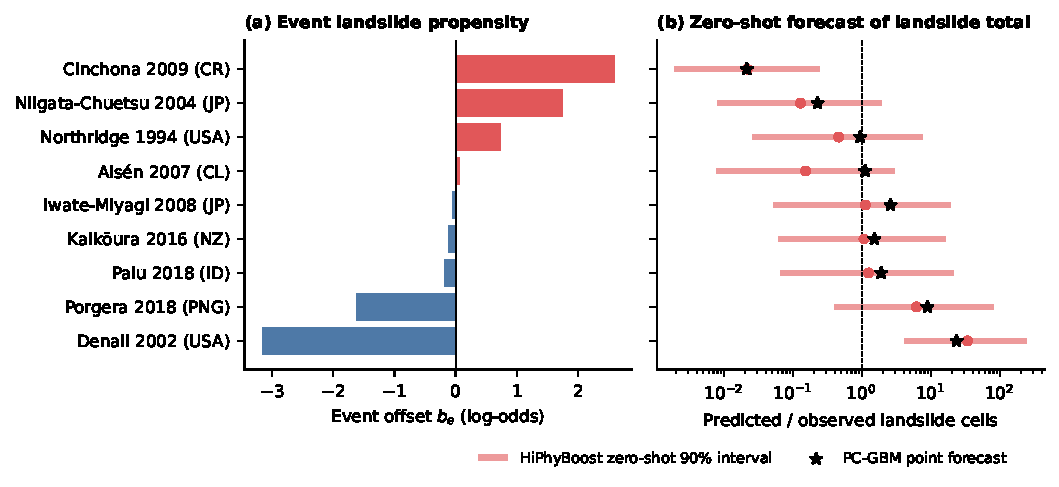
\includegraphics[width=\textwidth]{fig8_offsets.pdf}
\caption{(a) Event offsets $b_e$ of HiPhyBoost fitted on all nine earthquakes: the landslide propensity of each event relative to the population, with terrain and Newmark displacement held equal. (b) Zero-shot forecasts of the total number of landslide cells for each held-out event: HiPhyBoost 90\% predictive interval (bar) and median (dot), and the PC-GBM point forecast (star), all relative to the observed total (dashed line).}\label{fig:offsets}
\end{figure*}

\begin{figure*}[t]\centering
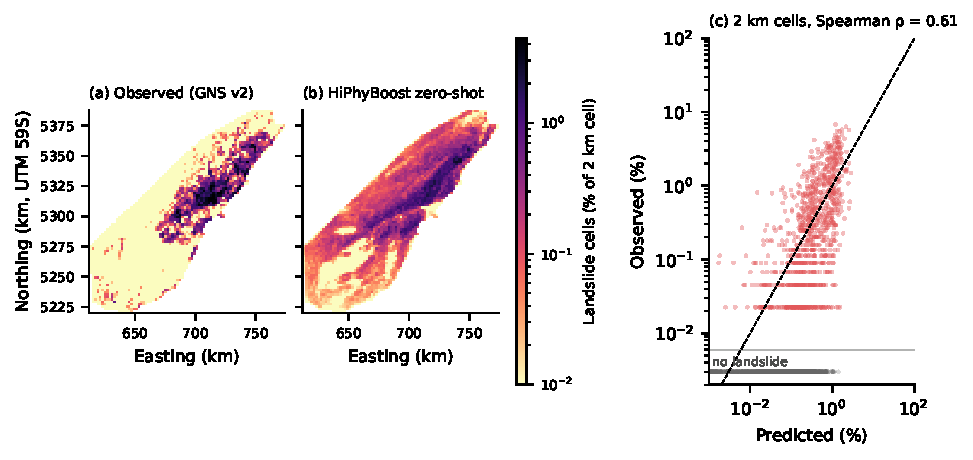
\includegraphics[width=\textwidth]{fig7_kaikoura_transfer.pdf}
\caption{Zero-shot transfer to the 2016 Kaik\={o}ura earthquake. (a) Observed percentage of 30~m cells containing a landslide source in 2~km cells (GNS Science inventory v2); (b) HiPhyBoost forecast trained only on the eight other Pacific Rim earthquakes (offset at the prior median); (c) predicted against observed density for 2~km cells; cells without any mapped landslide are shown in the bottom strip.}\label{fig:kaikoura}
\end{figure*}

\begin{figure*}[t]\centering
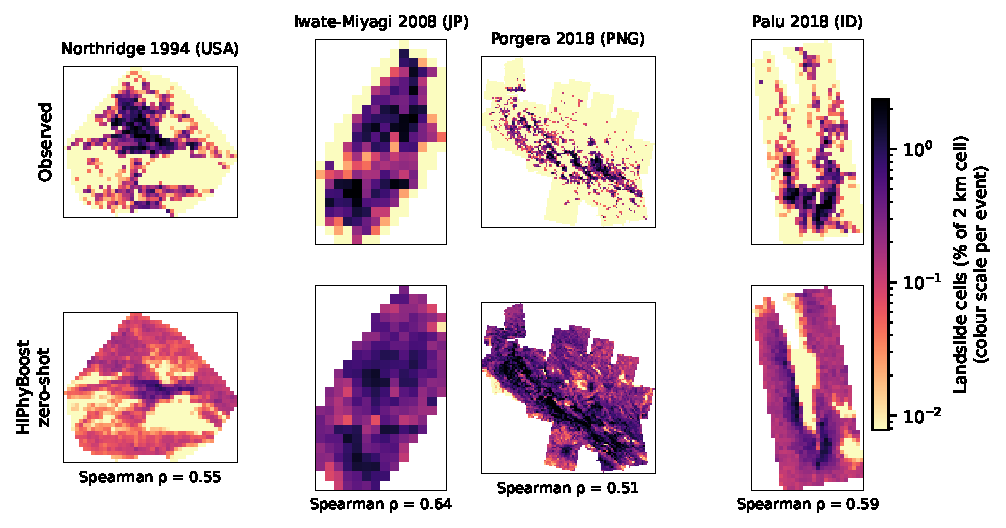
\includegraphics[width=\textwidth]{fig10_maps_multi.pdf}
\caption{Observed (top) and HiPhyBoost zero-shot (bottom) landslide density at 2~km resolution for four further held-out events. Each column uses its own colour scale; $\rho$ is the Spearman correlation between predicted and observed density over 2~km cells.}\label{fig:maps}
\end{figure*}
